\chapter{Аналитическая часть}

\section{Формализация задачи}
Объектами сцены являются:

\begin{enumerate}
    \item \textbf{подсолнухи};
    \begin{itemize}
        \item высота подсолнухов;
        \item количество подсолнухов на поле;
        \item амплитуда колебания подсолнухов под действием ветра;
        \item частота колебаний подсолнухов под действием ветра (количество колебаний в секунду).
    \end{itemize}

    \item \textbf{поле};
    \begin{itemize}
        \item ширина поля;
        \item длина поля;
        \item характеристики поверхности:
        \begin{itemize}
            \item рассеянное отражение;
            \item диффузное отражение.
        \end{itemize}
    \end{itemize}

    \item \textbf{источник света (солнце)};
    \begin{itemize}
        \item расположение: определяется по вертикальной траектории, имеющей форму круга.
    \end{itemize}

    \item \textbf{наблюдатель (камера)}.
    \begin{itemize}
        \item расположение;
        \item угол обзора.
    \end{itemize}
\end{enumerate}

Формализация задачи в виде IDEF0 представлена на рисунке~\ref{images:IDEF0}

\begin{figure}[H]
    \centering
    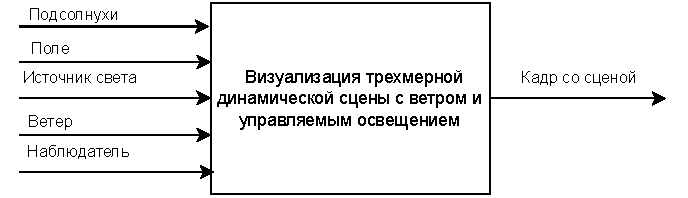
\includegraphics[width=130mm]{images/IDEF0}
    \caption{Формализациязадачи в виде IDEF0.}
    \label{images:generate_perms}
\end{figure}



\section{Алгоритмы для моделирования и визуализации природных объектов}

Для моделирования и визуализации природных объектов, таких как подсолнухи, существуют различные подходы и алгоритмы. Некоторые из них представлены ниже.


\subsection{Полигональное 3D-моделирование}
Полигональное моделирование — это метод создания трехмерных моделей с помощью полигонов, которые представляют собой плоские многоугольники, обычно треугольники или четырехугольники. Эти полигоны образуют сетку, которая формирует контур и поверхность объекта.~cite{lit1}

Преимущества:
\begin{itemize}
    \item высокая детализация: чем больше полигонов, тем более детализированной становится модель.
\end{itemize}

Недостатки:
\begin{itemize}
    \item сложность: требует значительного количества времени и усилий для создания сложных моделей;
    \item ограничения: может быть неэффективным для объектов с сложной внутренней структурой.
\end{itemize}

\subsection{Методы рендеринга}

\textbf{Scanline}
Метод рендеринга, который обрабатывает изображение построчно.

\textbf{Raytrace}
Этот метод симулирует путь света в реальном мире, отслеживая лучи, которые падают на объекты сцены и отражаются от них.

\textbf{Raycasting}
Упрощенная версия Raytrace, которая рассчитывает только первое столкновение луча с поверхностью.

\subsection{Выбор метода моделирования}
Для визуализации поля с подсолнухами было выбрано полигональное 3D-моделирование. Оно позволяет создавать детальные модели подсолнухов. Для рендеринга сцены был выбран метод Raycasting для баланса между скоростью и качеством изображения.



\section{Модели освещения}

В компьютерной графике модели освещения используются для имитации световых эффектов, когда свет аппроксимируется на основе физических законов. 

Основными параметрами, определяющими освещение, являются:
\begin{itemize}
    \item \textbf{свойства источников света}, включая их интенсивность и цвет,
    \item \textbf{свойства материала объекта}, такие как коэффициенты отражения, поглощения и пропускания света,
    \item \textbf{взаимодействие света с другими объектами} в сцене, например, затенение и переотражение,
    \item \textbf{цвет самой поверхности}, который определяется текстурами или параметрами материала.
\end{itemize}



\subsection{Модель Ламберта}

Модель Ламберта используется для расчета диффузного освещения. Формула освещения имеет вид:
\[
I = I_a + I_d \cdot \max(0, \vec{L} \cdot \vec{N}),
\]
где 
\( I_a \)~--- фоновая компонента, 
\( I_d \)~--- интенсивность источника света, 
\( \vec{L} \)~--- вектор направления света, 
\( \vec{N} \)~--- нормаль к поверхности.

\textbf{Достоинства}:
\begin{itemize}
    \item простота реализации,
    \item высокая скорость вычислений.
\end{itemize}

\textbf{Недостатки}:
\begin{itemize}
    \item не учитывает зеркальные отражения, что делает поверхность "матовой".
\end{itemize}



\subsection{Модель Фонга}

Модель Фонга включает три компоненты: фоновую, диффузную и зеркальную. 
Формула имеет вид:
\[
I = I_a + I_d \cdot \max(0, \vec{L} \cdot \vec{N}) + I_s \cdot \max(0, \vec{R} \cdot \vec{V})^n,
\]
где 
\( I_s \)~--- интенсивность зеркального света, 
\( \vec{R} \)~--- отражённый вектор, 
\( \vec{V} \)~--- направление к наблюдателю, 
\( n \)~--- параметр блеска.

\textbf{Достоинства}:
\begin{itemize}
    \item реализует блеск и блики,
    \item подходит для гладких поверхностей.
\end{itemize}

\textbf{Недостатки}:
\begin{itemize}
    \item зеркальная компонента может давать нереалистичные результаты при больших значениях параметра блеска.
\end{itemize}

\subsection{Модель Блинна-Фонга}

Модель Блинна-Фонга модифицирует зеркальную компоненту модели Фонга. Вместо отражённого вектора \( \vec{R} \) используется вектор полупути \( \vec{H} \), рассчитываемый как среднее между векторами света и наблюдателя:
\[
\vec{H} = \frac{\vec{L} + \vec{V}}{\|\vec{L} + \vec{V}\|}.
\]

Формула освещения:
\[
I = I_a + I_d \cdot \max(0, \vec{L} \cdot \vec{N}) + I_s \cdot \max(0, \vec{N} \cdot \vec{H})^n.
\]

\textbf{Достоинства}:
\begin{itemize}
    \item более естественные блики,
    \item ускорение расчётов.
\end{itemize}

\textbf{Недостатки}:
\begin{itemize}
    \item не подходит для анизотропных поверхностей.
\end{itemize}

\subsection{Модификация Wrap-around}

Модель Wrap-around улучшает модель Ламберта, добавляя дополнительный параметр \( k \), который позволяет источнику света освещать поверхность даже в затенённых областях:
\[
I_d = \max(k + (1 - k) \cdot (\vec{L} \cdot \vec{N}), 0).
\]

\textbf{Достоинства}:
\begin{itemize}
    \item улучшает реалистичность теней.
\end{itemize}

\textbf{Недостатки}:
\begin{itemize}
    \item увеличивает сложность расчётов.
\end{itemize}

\subsection{Выбор модели}

Для данной задачи подходящей является \textbf{модель Блинна-Фонга}. Она обеспечивает баланс между реализмом и производительностью. 

Эта модель:
\begin{enumerate}
    \item учитывает как диффузное, так и зеркальное освещение, что важно для создания реалистичного вида подсолнухов,
    \item даёт плавное распределение бликов,
    \item эффективнее модели Фонга за счёт упрощения расчёта зеркальной компоненты.
\end{enumerate}

Модель Ламберта слишком проста и не учитывает блеск поверхности, что делает её неподходящей для сцены с естественным освещением. Модификация Wrap-around не нужна, так как не требуется учитывать освещение затенённых областей.

Таким образом, \textbf{модель Блинна-Фонга} оптимально соответствует требованиям проекта, обеспечивая реалистичное освещение подсолнухов и высокую производительность.



\section{Алгоритмы удаления невидимых рёбер и поверхностей}

Ниже представлены некоторые из наиболее распространённых алгоритмов, их преимущества и недостатки.

\subsection{Алгоритм Робертса}

\textbf{Описание:} этот алгоритм работает в объектном пространстве и удаляет рёбра или грани, которые экранируются самим телом или другими объектами сцены. Требует, чтобы объекты были выпуклыми.

Преимущества:
\begin{itemize}
\item \textbf{точность:} позволяет точно определить видимые рёбра;
\item \textbf{простота реализации:} использует простые математические методы.
\end{itemize}

Недостатки:
\begin{itemize}
\item \textbf{высокая вычислительная сложность:} объём вычислений растёт как квадрат числа объектов;
\item \textbf{ограничение на невыпуклые объекты:} требует разбиения невыпуклых объектов на выпуклые части~\cite{lit1, lit2, lit5}.
\end{itemize}

\subsection{Алгоритм Аппеля}

\textbf{Описание:} вводит понятие количественной невидимости, когда рёбра классифицируются по количеству граней, их закрывающих.~\cite{lit3}.

Преимущества:
\begin{itemize}
\item упрощение анализа: позволяет упростить анализ видимости рёбер.
\end{itemize}

Недостатки:
\begin{itemize}
\item ограниченное применение: в основном используется для контурных линий и не подходит для всех типов объектов
\end{itemize}

\subsection{Z-буфер}

\textbf{Описание:} работает в пространстве изображения и использует буфер глубины для определения видимости пикселей. Каждый пиксель проверяется на глубину, чтобы определить, какой объект ближе к наблюдателю.~\cite{lit3, lit4}

Преимущества:
\begin{itemize}
\item эффективность: быстрый и широко поддерживается современными видеокартами.
\end{itemize}

Недостатки:
\begin{itemize}
\item ограниченная точность: может давать ошибки при определении видимости в сложных сценах.
\end{itemize}

\subsection{BSP-деревья}

\textbf{Описание:} используются для оптимизации рендеринга статических сцен путём разбиения пространства на более мелкие части и определения видимости объектов.~\cite{lit3}

Преимущества:
\begin{itemize}
\item эффективность: позволяет быстро исключать невидимые объекты;
\item применение в сложных сценах: подходит для архитектурных и других статических сцен.
\end{itemize}

Недостатки:
\begin{itemize}
\item сложность реализации: требует значительных усилий для построения и обновления дерева;
\item ограниченное применение: в основном используется для статических сцен.
\end{itemize}

\subsection{Иерархический Z-буфер}

\textbf{Описание:} разделяет z-буфер на более мелкие части для более эффективного удаления невидимых поверхностей.~\cite{lit3}

Преимущества:
\begin{itemize}
\item улучшенная эффективность: позволяет быстрее исключать невидимые треугольники;
\item применение в сложных сценах: подходит для больших сцен с множеством объектов.
\end{itemize}

Недостатки:
\begin{itemize}
\item Сложность реализации: Требует ручного обновления пирамиды при добавлении новых объектов.
\item Высокие требования к памяти: Для хранения иерархии z-буфера.
\end{itemize}

\begin{table}[H]
\small
\centering
\resizebox{\textwidth}{!}{ % Масштабируем таблицу по ширине страницы
\begin{tabular}{|l|c|c|c|} % Убедитесь, что количество столбцов соответствует данным
\hline
\textbf{Алгоритмы} & \textbf{Поддержка} & \textbf{Поддержка} & \textbf{Требования} \\ 
\textbf{} & \textbf{сложных сцен} & \textbf{дин. объектов} & \textbf{к памяти} \\ \hline
\textbf{Алг. Робертса} & Нет & Нет & Низкие \\ \hline
\textbf{Алг. Аппеля} & Нет & Нет & Низкие \\ \hline
\textbf{Z-буфер} & Да & Да & Средние \\ \hline
\textbf{BSP-деревья} & Да (для стат.) & Нет & Высокие \\ \hline
\textbf{Иерарх. Z-буфер} & Да & Да & Высокие \\ \hline
\end{tabular}
}
\caption{Сравнение алгоритмов удаления невидимых рёбер и поверхностей}
\label{tab:comparison}
\end{table}



Для реализации поставленной задачи наиболее подходящим методом является Z-буфер. Он поддерживает сложные сцены с динамиескими объектами.


\section{Скелетная Анимация}

Скелетная анимация — это метод создания движений в трехмерных моделях, который использует внутренний «скелет» для управления деформацией и движением объекта. Этот скелет состоит из костей и суставов, которые функционируют аналогично человеческому скелету, позволяя аниматорам создавать реалистичные и плавные движения~cite{lit2}.

\subsection{Механизм работы костей}

\begin{itemize}
    \item \textbf{Создание скелета:} аниматоры создают набор костей, которые соединены между собой суставами. Каждая кость может двигаться относительно других костей, что позволяет создавать сложные движения. Например, для моделирования руки человека создаются кости для плеча, предплечья и кисти, соединенные суставами. Это позволяет анимировать руку, сгибая её в локте или вращая кисть.
    
    \item \textbf{Привязка модели (скиннинг):} модель привязывается к скелету, что позволяет каждому полигону модели быть привязанным к определённой кости. Этот процесс называется скиннингом. Каждая вершина модели может быть привязана к одной или нескольким костям с определёнными весами. Веса определяют, насколько сильно каждая кость влияет на вершину. 
    Формула для вычисления новой позиции вершины:
    
\[
\mathbf{v}' = \sum_{i=1}^{n} w_i \cdot \mathbf{T}_i \cdot \mathbf{v},
\]
где:
\begin{itemize}
    \item \(\mathbf{v}\) — исходная позиция вершины,
    \item \(\mathbf{v}'\) — новая позиция вершины,
    \item \(w_i\) — вес вершины для \(i\)-й кости,
    \item \(\mathbf{T}_i\) — матрица преобразования \(i\)-й кости,
    \item \(n\) — количество костей, влияющих на вершину.
\end{itemize}
    Этот процесс позволяет модели деформироваться в соответствии с движением костей.
    
    
    \item \textbf{Анимация:} движения костей определяются с помощью ключевых кадров, которые задают положение и вращение костей в определенные моменты времени. Программа интерполирует промежуточные кадры, создавая плавные движения. Для интерполяции часто используется линейная или сплайновая интерполяция. 
    Формула линейной интерполяции:
    \[
\mathbf{q}(t) = (1 - t) \cdot \mathbf{q}_1 + t \cdot \mathbf{q}_2,
\]
где:
\begin{itemize}
    \item \(\mathbf{q}_1\) и \(\mathbf{q}_2\) — ключевые кадры,
    \item \(t\) — параметр интерполяции (\(0 \leq t \leq 1\)).
\end{itemize}
Этот подход позволяет аниматору задавать только ключевые позы, а программа автоматически вычисляет промежуточные состояния.
\end{itemize}



\subsection{Визуализация ветра}

Для симуляции воздействия ветра на объекты, такие как растения, можно использовать математическую модель, которая описывает силу ветра как функцию времени и пространства.
Рассмотрим функцию ветра:
\[
F(t) = A \cdot \sin(2\pi f t + \phi),
\]
где:
\begin{itemize}
    \item \(A\) — амплитуда силы ветра,
    \item \(f\) — частота колебаний,
    \item \(\phi\) — фаза колебаний,
    \item \(t\) — время.
\end{itemize}

Эта функция описывает периодическое воздействие ветра. В таком случае, для симуляции колыхания стебля растения под воздействием ветра, угол поворота кости может быть вычислен по формуле:

\[
\theta(t) = k \cdot F(t),
\]
где:
\begin{itemize}
    \item \(k\) — коэффициент, зависящий от гибкости кости,
    \item \(F(t)\) — сила ветра в момент времени \(t\).
\end{itemize}

Для визуализации ветра скелетная анимация может быть полезна по нескольким причинам:

\begin{itemize}
    \item \textbf{Реализм движений:} скелетная анимация позволяет создавать реалистичные и плавные движения.
    
    \item \textbf{Эффективность:} после создания скелета и привязки модели анимацию можно быстро создавать, используя инструменты интерполяции между ключевыми кадрами. Это ускоряет процесс анимации.
    
    \item \textbf{Гибкость:} скелетная анимация позволяет легко изменять позы и движения объектов, что дает воможность легко управлять положением отдельных частей модели для создания более сложной анимации.
\end{itemize}

\subsection{Применение в визуализации ветра}

Хотя скелетная анимация обычно используется для персонажей, она также может быть применена к растениям или другим объектам, на которые воздействуют внешние силы (например, ветер). Для этого создается скелет, который имитирует стебли растения, и привязывается к ним модель листьев и других элементов. Движения костей позволяют симулировать колыхание растений под воздействием ветра, создавая реалистичную и динамичную сцену.


\section{Описание модели подсолнуха}
Для выполнения поставленной задачи визуализации трехмерной сцены поля подсолнухов была выбрана модель подсолнуха в формате FBX. Данная модель была выбрана благодаря своей высокой детализации и наличию встроенного скелета, состоящего из костей.

 На рисунке~\ref{images:Blender} представлена модель подсолнуха, загруженная в программу Blender. На изображении отображены основные компоненты модели, включая геометрию объекта и структуру скелета, состоящего из костей, которые используются для анимации.

 На рисунке~\ref{images:Real} показана модель подсолнуха в процессе выполнения программы.


\begin{figure}[H]
    \centering
    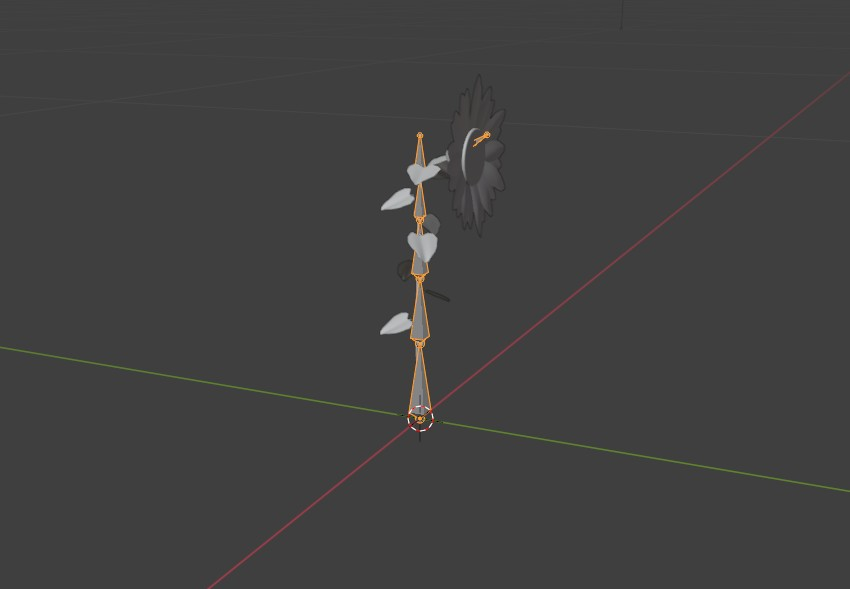
\includegraphics[width=130mm]{images/Blender}
    \caption{Модель подсолнуха, загруженная в программу Blender}
    \label{images:Blender}
\end{figure}

\begin{figure}[H]
    \centering
    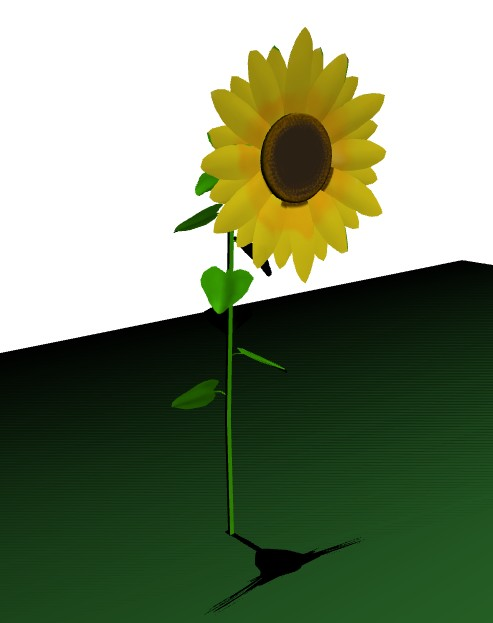
\includegraphics[width=110mm]{images/Real}
    \caption{Модель подсолнуха в процессе выполнения программы.}
    \label{images:Real}
\end{figure}